%%%%%%%%%%%%%%%%%%%%%%%%%%%%%%%%%%%%%%%%%%%%%%%%%%%%%%%%%%%%%%%%
% Guide
%%%%%%%%%%%%%%%%%%%%%%%%%%%%%%%%%%%%%%%%%%%%%%%%%%%%%%%%%%%%%%%%
\section{预测校正制导}
理论上当大气入口条件和变轨目标确定后,
即可得出一条确定轨迹,气动飞行期间不用施加控制即可实现既定的捕获任务。
但实际飞行中存在极强的环境不确定性,飞行器及进入轨道本身也存在初始条件的不确定性,因此需要设计在轨制导律。
气动飞行的制导方法主要分为标称轨迹制导和预测校正制导。
制导算法的鲁棒性也是需要重点考虑的问题关键,在不确定性强的环境下,
预测校正制导相对标称轨迹的解析制导更具备优势\cite{dqingyuan2019}。
在轨制导律的控制量输出是倾侧角随时间变化的函数,
如果控制器离散,则输出的是倾侧角序列。
原文使用的是离散的全系数自适应控制。

原文中提出了一种标称制导和两种预测校正制导方法。
标称制导指的是在假设没有各种随机因素影响的情况下,
以总速度增量最小或能量最小为目标的最优控制,
生成的倾侧角序列为先以最小倾侧角飞行,
再以最大倾侧角飞行,此时能量最优。
两种预测校正制导方法的控制律相同,但制导目标不同。
一种是目标远拱点误差,也就是以实际远点高度与设定的远点高度的差作为评价指标;
另一种是远拱点抬升速度增量,也就是在近拱点处开启发动机调整远拱点时,以速度增量大小作为评价指标。
本文复现第一种目标。

制导部分被控对象的输入是远拱点误差,输出是倾侧角。
在离散控制器的每个更新时刻,计算如果保持当前输入的倾侧角指令不变,
飞行器飞出大气层后以当前的位置和速度向量换算成轨道元素,进而求出远拱点误差。

被控对象的特征模型为
\[ y(k) = \alpha_1(k)y(k-1) + \beta_0(k)u(k) \]
预测校正制导的控制律使用线性反馈控制:
\begin{align}
    &u(k) = u(k-1) + u_L(k) \notag\\
    &u_L(k) = -\frac{l_1\alpha_1(k)y(k)}{\beta_0(k)} \label{eqGuideCtrl}
\end{align}
其中控制量$u_L(k)$为一个倾侧角余弦变化量$\Delta\cos\sigma$。
第一种制导目标中,
\begin{equation*}
    \Delta r = r_a^e(k) - r_a^*
\end{equation*}

因为输出的数值变化范围可能达到$10^4$km数量级,
但又需要把输出映射到$\cos\sigma$,也就是$[-1,1]$的范围内,
所以需要进行输入变换,将远拱点误差乘一个系数。
“当前时刻施加的$\Delta\cos\sigma(k)$对最终过渡轨道远拱点半径$r_a^e(k)$的影响是一个和时间有关的函数,
且越早施加的改变量对最终轨道影响越大”\cite{dqingyuan2019}。
因此该系数需要实时计算。
输入和输出的关系为
\begin{equation}
    \Delta r = f(\Delta\cos\sigma) \label{eqGuideFunc}
\end{equation}
也就是说远拱点误差是倾侧角的垂直分量的函数。
定义输入变换系数为式\eqref{eqGuideFunc}的泰勒展开的一阶项
\begin{equation*}
    A(k) = \frac{\partial r(k)}{\partial\cos\sigma(k)}
    \cong \frac{\Delta r(k) - \Delta r^+(k)}{\cos\sigma(k) - \cos(\sigma(k)+10^\circ)}
\end{equation*}
其中$\Delta r^+(k)$是施加$\sigma(k)+10^\circ$倾侧角的情形下最终过渡轨道的远拱点误差。
这样,将式\eqref{eqGuideCtrl}中的$y(k)$施加动态输入变换
\[y(k) = \frac{\Delta r}{A(k)}\]
再取合适的制导律参数$l_1$即可将控制量$u_L(k)$限制在一个合适的区间内。
制导整体框图如图\ref{figGuideSketch}所示。
\begin{center}
	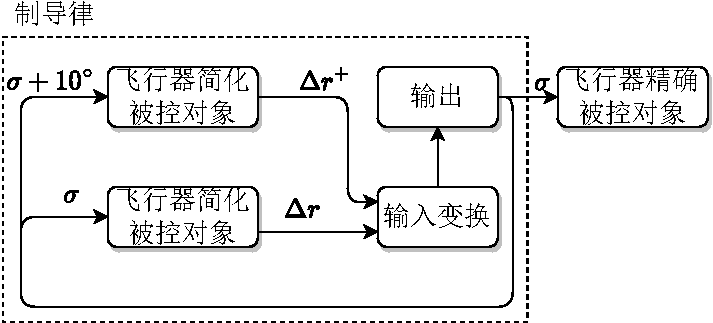
\includegraphics[scale=0.7]{GuideSketch.pdf}  \\
	\figcaption{制导整体框图}\label{figGuideSketch}
\end{center}

$10^\circ$是原文数据,本文为方便起见统一采用弧度制。
我认为既然是增量那就应该取一个极小量,不清楚作者取$10^\circ$这么大数字的原因。
另外考虑到倾侧角过大会导致简化模型的预测中可能出现高度过低甚至与火星相撞的情况,
因此将弧度增量取负,由$10^\circ$改为$-10^{-3}$rad。

侧向制导与纵向制导独立,
如果侧向速度太快,翻转倾侧角即可,大致原理如图\ref{figGuideSide}所示。
\begin{center}
	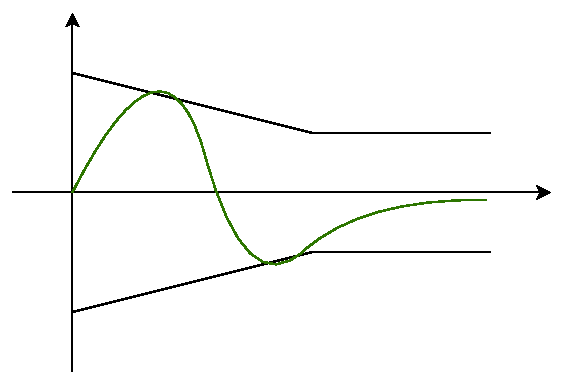
\includegraphics[scale=0.7]{GuideSide.pdf}  \\
	\figcaption{侧向制导翻转倾侧角原理}\label{figGuideSide}
\end{center}
同样因为倾侧角对远拱点半径的影响不是定值,所以翻转阈值需要越来越小。
原文使用一次函数,我认为大气层内飞行的时间不是定值,
所以采用了指数衰减函数。

纵向制导和侧向制导理论上分别研究的是$L\cos\sigma$和$L\sin\sigma$,
两者能够独立分析的原因是原文侧向制导实际上只研究了符号,
此外,直接翻转倾侧角会消耗大量的燃料改变姿态,
并且原文中使用离散制导律更新控制量也造成了离散的倾侧角状态,
我认为这3种因素都导致了燃料消耗不是最优解,此处存在疑问。
